Weinberg第二章,讲述相对论性的量子力学!这一章,我们的核心就是说明,量子场论是唯一合理的融合相对论和量子力学的方法。因而我们从量子力学开始进行讨论。    

\section{量子力学基本概念}
量子力学是由下面几个公里体系进行构建的:
\bigskip

\textbf{1. 量子态由Hilbert空间的ray描述}
\defi{
我们定义Hilbert空间:

\itm{
    \pt{复线性空间「也就是线性组合的系数是复数」}
    \pt{并且其上可以定义一个norm,满足:}
    \eq{
    \begin{gathered}(\Phi,\Psi)=(\Psi,\Phi)^*,\\(\Phi,\xi_1\Psi_1+\xi_2\Psi_2)=\xi_1(\Phi,\Psi_1)+\xi_2(\Phi,\Psi_2),\\(\eta_{1}\Phi_{1}+\eta_{2}\Phi_{2},\Psi)=\eta_{1}^{*}(\Phi_{1},\Psi)+\eta_{2}^{*}(\Phi_{2},\Psi).\end{gathered}
}
    \pt{这个norm是有正定条件: $ \braket{\Psi}{\Psi} \geq 0$,并且当且仅当 $ \Psi =0 $取等  }
}
}
在这个空间上我们可以定义ray:
\itm{
    \pt{自己内积为1的向量集合 $ \braket{\Psi}{\Psi} = 1 $ }
    \pt{同时模去所有 $ \Psi' = \xi i \Psi  $ 其中 $ \xi $是模长为1的复数 }
}

\textbf{2. 可观测量由Hermite算符描述}

所有客观测量都可以理解为一个Hilbert空间到自己的映射,需要满足下面条件:
\itm{
    \pt{映射是线性的:$ A(\xi\Psi+\eta\Phi)=\xi A\Psi+\eta A\Phi $ }
    \pt{映射是Hermite的,也就是对于内积结构需要满足 $ A^\dagger=A $ 。其中Hermite共轭定义为:$ (\Phi,A^\dagger\Psi)\equiv(A\Phi,\Psi)=(\Psi,A\Phi)^*. $ }
}
\rmk{注意Hermite这个特性是基于内积结构的。只有定义了合理的线性空间的内积结构我们才能定义Hermite的映射}

对于一个量子态来说,如果这个量子态对应的ray里面所有向量都是客观测量算符A得本征向量,我们可以得到A的对于一个态的具体数值:
\eq{
    A\Psi=\alpha\Psi\quad\mathrm{for}\quad\Psi\mathrm{~in~}\mathscr{R}.
}
同时根据Hermite的算符的特性:
\itm{
    \pt{得到的数值 $ \alpha $是实数 }
    \pt{不同的特征值对应的特征向量都是正交的,也就是对于内积结构是0。}
}

\textbf{3. 实验结果}

对于一个ray R所代表的量子态。实验意味着检测这个态在不在某一组正交的 $ \{R_1,R_2,R_3,...\} $中的某一个量子态上。并且发现这个量子态在另外一个量子态上面的概率是:
\eq{
    \mathcal{P}(\mathscr{R}\to\mathscr{R}_n)=\left|(\Psi,\Psi_n)\right|^2,
}  
其中 $ \Psi $和$ \Psi_n $ 是这个量子态的ray上面的任意两个矢量。\textbf{注意,这也是为什么我们要最后取模长平方,因为我们要消除ray的香味的影响。} 

如果我们有一组不仅仅是正交而且是完备的ray的基,进行测量「也就是对于Hilbert空间能够span整个空间」,那么我们测量得到不同结果的概率应该满足:
\eq{
    \sum_nP(\mathscr{H}\to\mathscr{H}_n)=1
}

\tip{没有薛定谔方程}{
    我们发现我们这里根本没有在量子力学的公理里面提及薛定谔方程。因为这个那本不是本质的内容。

    时间演化也还是一种对称性变换。对于相对论量子力学应该在考虑量子力学的对称性变化的时候考虑。
}

\section{对称性变换Symmetry}

\subsection{对称性变换算符}
\imp{对称性变换是什么}{所谓对称性变换,就是我们改变观察者的状态,这并不会影响实验结果。比如:我们认为,跑着和站着观察,实验结果是一模一样的。

所有我们认为不改变物理规律本身的变换其实都是对称性变换。比如:观察者的移动emmm}
我们考虑不同观察者进行同样的一组测量「物理意义上的【同样】,就是干一样的事情」。
\itm{
    \pt{对于观察者O来说,这个系统使用R量子态描述,我们希望进行测量于 $ \{R_1,R_2,...\} $量子态上}
    \pt{对于观察者O'来说,这个系统使用R'量子态描述,我们希望进行测量于 $ \{R_1',R_2',...\} $量子态上}
}
那么测量给出的概率一定是相通的:
\eq{
    P(\mathscr{R}\to\mathscr{R}_n)=P(\mathscr{R}^{\prime}\to\mathscr{R}_n^{\prime}).
}
\rmk{注意这个仅仅是是对称性变换的必要条件,也就是满足这个性质的变换必然是对称性变换,但是对称性变换还有其它种。}
\thm{
  对称性变换在Hilbert空间的表示(Wigner)

  对于对称性变换来说,对应Hilbert空间上的算符U,将Hilbert空间上所有向量$ \Psi $ 变换为:$ U \Psi $。这个算符只能是两种可能:
  \itm{
    \pt{线性并且Unitary}
    \eq{
        (U\Phi,U\Psi)=(\Phi,\Psi),\quad
        U(\xi\Phi+\eta\Psi)=\xi U\Phi+\eta U\Psi
    }
    \pt{反线性且antiunitary}
    \eq{
        (U\Phi,U\Psi)=(\Phi,\Psi)^*,\quad U(\xi\Phi+\eta\Psi)=\xi^*U\Phi+\eta^*U\Psi
    }
  }
}
我觉得有两种情况是因为,我们的概率是模长平方,所以可能会有问题。
\rmk{我们定义的可观测量都是线性算符,但是对称性变换的算符可以是线性的也可以是反线性的。并且一个需要时Hermite的,另一个需要的是Unitary!这是两个不一样的条件。}
\rmk{注意,反线性其实说的就是常数和算符在交换的时候会变成复共轭,所以\textbf{我们一定不要默认常数和算符永远是对易的,如果是反线性的算符会出现复共轭的问题}}
我们注意到我们上面使用的定义没有使用 $ U^{\dagger} $进行定义,因为线性和反线性的算符的共轭的定义是不同的。我们需要给出两者的定义才能使用这个符号
\itm{
    \pt{对于线性算符,我们定义Hermite共轭是:$ (\Phi,L^\dagger\Psi)\equiv\left(L\Phi,\Psi\right). $ }
    \pt{对于反线性算符,我们不能这么定义,我们如果用两个态展开$ \Phi $就会推出矛盾。所以对于反线性算符我们定义为:$ (\Phi,A^\dagger\Psi)\equiv(A\Phi,\Psi)^*=(\Psi,A\Phi) $ }
}
在此基础上,我们知道Unitary条件可以对于线性和反线性算符使用同样的一个表达式写出:
\eq{
    U^\dagger=U^{-1}.
}


但是,下面我们知道,由于Identity算符显然是一个对称性变换的算符,并且对称性变换我们要求是连续的。所以所有的算符都应该是Identity算符连续变换得到的。所以我们认为:
\imp{对称性变换}{
    所有的对称性变换可以通过线性并且是Unitary的算符描述。
}
\rmk{所有反线性的变换算符,也可以描述对称性变换,但是,他们一般描述的变换都存在时间反演的变换。}

\textbf{无限小对称性变换}

都可以使用下面这样的形式进行描述:
\eq{
    U=1+\mathrm{i}\epsilon t
}
其中t需要是一个Hermite的算符才能保证U是一个Unitary的算符。而 $ \epsilon $是一个无限小的实数。 

\subsection{对称性变换和群表示}

一般所有的对称性变换存在群结构。我们可以定义Unitary矩阵的乘法「群元素的乘法」;Unitary矩阵的逆「群元素的逆元」;Idenity「群的Identity」。

但是一个特别注意的事实是,由于我们表示量子态是一个ray。所以我们群乘法来说,可能会有一个相位的ambiguity,也就是对于两个对称性变换 $ T_1,T_2 $,他们对应的对称性变换Unitary算符的乘法,和他们的复合对应的对称性算符可能差了相位:
\eq{\label{eq:phase}
    U(T_2)U(T_1)\Psi_n=e^{i\phi_n(T_2,T_1)}U(T_2T_1)\Psi_n.
}
\lmm{
  相位与量子态无关

    \textbf{除了一种重要的特殊情况},由于\textbf{算符的线性性},\textbf{这个相位和作用的态没有关系,仅仅和对称性变换本身有关}。

    证明:
\eq{
    \begin{aligned}e^{\mathrm{i}\phi_{AB}}U(T_{2}T_{1})(\Psi_{A}+\Psi_{B})&=U(T_2)U(T_1)(\Psi_A+\Psi_B)\\&=U(T_2)U(T_1)\Psi_A+U(T_2)U(T_1)\Psi_B\\&=e^{\mathrm{i}\phi_A}U(T_2T_1)\Psi_A+e^{\mathrm{i}\phi_B}U(T_2T_1)\Psi_B.\end{aligned}
}
我们在等式两遍乘上,U的逆,我们就可以得到:
\eq{
    e^{\pm i\phi_{AB}}(\Psi_A+\Psi_B)=e^{\pm i\phi_A}\Psi_A+e^{\pm i\phi_B}\Psi_B,
}
因此之后相位和量子态无关的时候才能成立。所以我们才能写作 \cref{eq:phase}的形式。
}

\textbf{讨论1:并非严格群表示而是projective rep}

所以其实U\textbf{并不是严格满足群的变换关系},只是$ \phi = 0 $的时候才严格作为一个对称性变换群的表示。数学上,差个相位被称为:projective representation。一般的李群的结构能够告诉我们这个群是否有projective rep。所以我们就知道他对应的对称性变换算符会不会是projective的。
\bigskip

\textbf{讨论2:上方证明的例外}

例外的情况是,有的时候两个态是不能够进行叠加的。
\rmk{原则上Hilbert空间上的向量都是可以进行叠加的。但是有一些叠加的方式我们认为是non-physical的。

一个重要的例子就是,整数和半整数自旋的态是不能够进行叠加的。同样的,对于一个表示\textbf{如果我们计算出来相位和某一个物理量有关,那么,我们知道,这个物理量不同的量子态是不能够进行叠加的。}
}
这样的话,对于不能互相叠加的态,我们可以分成很多类,每一类可以有自己的一个独特的相位。\textbf{但是我们也知道,对于一个有projective rep的李群来说,这个群可以进行扩展成为一个所有表示都可以是non-projective的群。}所以我们目前可以只考虑 $ \phi = 0 $的情况。 
\subsection{Connected Lie Group}

存在一系列群,联通李群,对于物理十分重要。这个群存在两个特别特殊的性质:
\itm{
    \pt{这个群的元素可以用一组有限多个实数进行描述 $ \theta^\alpha $。并且每一个元素都和Identity是道路联通的。 }
    \pt{这个群的复合可以使用这样的函数进行描述: $ T(\bar{\theta})T(\theta)=T\left(f(\bar{\theta},\theta)\right) $ ,其中函数满足,当一个$ \theta $是0的情况下:$ f^a(\theta,0)=f^a(0,\theta)=0^a. $ \textbf{ 对于联通李群我们可以定义复合关系 $ f(\bar{\theta},\theta) $ }}
}
\imp{复合规则}{
    对于一个联通李群来说,由于我们已经很熟悉$ \mathbb{R}^n $,我们这个群的【复合规则】实际上给出了一个从$ \mathbb{R}^n $到群的映射。所以\textbf{复合规则描述了群的所有结构。} 
}
\rmk{这里需要提示:f 是一个从 $ \mathbb{R}^n \times \mathbb{R}^n  $到 $ \mathbb{R}^n $的映射,其中n的取值就是 $ \alpha $ 有多少个!! 

并且注意对于复合规则这件事:$ f(\bar{\theta},\theta) $ 的映射可以定义是因为这个群元素是由 $ \mathbb{R}^n $空间进行描述的。所以,后面讨论这个f的都是对于由这样复合规则的群来说的。 
}
对于一个联通李群来说,我们可以对于对称性变换算符进行展开:
\eq{\label{eq:expansiont}
    U\left(T(\theta)\right)=1+i\theta^at_a+\frac{1}{2}\theta^b\theta^ct_{bc}+\cdots,
}
其中 $ t_a $和 $ t_{bc} = t_{cb} $都是由几个指标标定的Hermite的算符,并且这个算符是一个常数,相当于展开的系数。当我们认为这个对称性算符给出了李群的表示(而不是projective rep)的时候,$ U\left(T(\bar{\theta})\right)U\left(T(\theta)\right)=U\left(T(f(\bar{\theta},\theta))\right). $ 我们假设 $ f(\bar{\theta},\theta) $ 函数可以进行下面的展开:
\eq{
    f^{a}(\bar{\theta},\theta)=\theta^{a}+\bar{\theta}^{a}+f^{a}{}_{bc}\bar{\theta}^{b}\theta^{c}+\cdots
} 
\textbf{注意,我们这个展开没有$ \theta^2 $项,否则就不能满足第二个条件了。 }
我们对比左右两边的式子:
\eq{
    \begin{aligned}
        &U(T(\bar{\theta}))U(T(\theta)) = \begin{bmatrix}1+i\bar{\theta}^at_a+\frac{1}{2}\bar{\theta}^b\bar{\theta}^ct_{bc}+\cdots\end{bmatrix}\times\begin{bmatrix}1+i\theta^at_a+\frac{1}{2}\theta^b\theta^ct_{bc}+\cdots\end{bmatrix}\\=&1+i\left(\theta^a+\bar{\theta}^a+f_{bc}^a\bar{\theta}^b\theta^c+\cdots\right)t_a+\frac{1}{2}(\theta^b+\bar{\theta}^b+\cdots)(\theta^c+\bar{\theta}^c+\cdots)t_{bc}+\cdots\\
        = &U(T(f(\bar{\theta },\theta)))
    \end{aligned}
}
我们给出:
\pict{2025-07-07-17-50-26.png}{0.55}
因此有一个nontrivial的结论就是:
\eq{\label{eq:nontritwo}
    t_{bc}=-t_{b}t_{c}-if^{\alpha}{}_{bc}t_{a}.
}
也就是说,我们的$ f^a_{bc} $给定,也就是给定李群的结构,二阶的展开的Hermite矩阵$ t_{bc} $完全由一阶的矩阵$ t_a $决定。 

此外,有一个consistency的条件也就是,$ t_{bc} $对于两者指标必须是对称的,因为这个相当于二阶的泰勒展开的导数,需要时对称的。所以我们根据\cref{eq:nontritwo}之中$ t_{bc} = t_{cb} $ 得到我们的一阶的Hermite矩阵需要满足下面的关系:
\eq{\label{eq:algebra}
    [t_b,t_c]=iC^a{}_{bc}t_a,
}
其中,$ C^a{}_{bc} $ 被称为结构常数,可以被下面求出来:
\eq{
    C^a{}_{bc}\equiv-f^u{}_{bc}+f^u{}_{cb}.
}
像是这样的对易关系\cref{eq:algebra}我们称之为李代数。
\imp{李代数结构}{
    下面我们将会知道,存在一系列类似于\cref{eq:nontritwo}的恒等式,让我们可以通过李代数的\textbf{生成元} $ t_a $ 得到所有的展开系数。

    注意,我们并不是得到所有$ \theta $取值下面的$ U(T(\theta)) $,而是,这个算符在Identity附近的一个临域内的展开。  
}
\bigskip

\textbf{Abelian group}

存在一种特殊情况就是,$ f^u(\theta,\bar{\theta})=\theta^a+\bar{\theta}^a. $ 线性的情况下,我们会发现,$ f^a{}_{bc} = 0 $并且同时也就满足:$ [t_b,t_c] = 0 $。这样的群我们称为 \textbf{Abelian group}。对于这样的群,我们知道f复合只是单纯的相加,所以我们可以把很多很小的 $ \theta $ 加在一起。并对于这些很小的加和取极限,给出:
\eq{\label{eq:dedec}
    U\left(T(\theta)\right)=\left[U\left(T\left(\frac{\theta}{N}\right)\right)\right]^N = \lim_{N\to\infty}\left[1+\frac{i}{N}\theta^at_a\right]^N
}
根据指数函数的定义,我们会发现,对于Abelian的群来说,对应的所有对称性算符都需要满足下面的形式:
\eq{\label{eq:ablianr}
    U\left(T(\theta)\right)=\exp(it_a\theta^a)\mathrm{~.}
}
\rmk{这里我们学到了什么呢?
\itm{
    \pt{一系列对称性变换是通过联通李群进行描述的,是联通李群的表示}
    \pt{联通李群存在李代数结构,并且其行为可以很大程度在Identity附近被李代数描述。}
}
}
\tip{指数算符关系}{
    其实算符写作$  U\left(T(\theta)\right)=\exp(it_a\theta^a)\mathrm{~.} $的形式并不一定是要求整个完整的群是Abelian的。
    
    而是,当群有一个Abelian的子群「并且包含Identity」那么就是可以写作这个形式。一般的常见的群其实都能够进行这个操作。比如:对于旋转群,虽然不是Abelian的,但是存在「绕固定轴旋转」这个子群,所以我们对于旋转群的元素对应的算符依旧可以写作这个形式。
}

\section{量子Lorentz变换}

\textbf{狭义相对论告诉我们不同惯性系之间存在着一个特殊的坐标变换}
\imp{惯性系坐标变换}{
    惯性系之间坐标变换需要满足,对于不同的惯性系我们可以赋予直角坐标系,其坐标系分量需要满足:
\eq{\label{eq:lorentz}
    \eta_{\mu\nu}dx^{\prime\mu}dx^{\prime\mu}=\eta_{\mu\nu}dx^{\mu}dx^{\nu}
}
这里我们使用的记号$ \eta_{\mu\nu} $ 是一个矩阵,这个矩阵是对角的且满足:
\eq{
    \eta_{11}=\eta_{22}=\eta_{33}=+1,\quad\eta_{00}=-1
}
这样的坐标变换保证了光速在所有的坐标系都是不变的。并且光速是1。
}
\rmk{上面的式子很让人困惑,因为这是一个记号。我们有两种理解这个微元的方式:

1. 积分起来的结果:

我们把两边积分起来就是 $ x^2- t^2 $。所以这个变换定义的是任意两个事件的时空间隔是不变的。

2. 求导的结果:

坐标变换矩阵保持lorentz signature的存在,也就是:
\eq{
    \eta_{\mu\nu}\frac{\partial x^{\prime\mu}}{\partial x^\rho}\frac{\partial x^{\prime\mu}}{\partial x^\sigma}=\eta_{\rho\sigma}.
}
其中,$ \frac{\partial x^{\prime\mu}}{\partial x^\rho} $ 就是坐标变换的求导。
}

% \rmk{我们定义的 $ \eta_{\mu\nu}dx^{\mu}dx^{\nu} $其实是时空的间隔,为什么是时空间隔不变可以推倒出光速不变呢?因为,在某一个参考系之中光的世界线的是空间间隔永远是0,由于是空间隔不变,所以光在其他参考系的世界线的速度也是1.所以这样的参考系变换下,光速永远是不变的。}
\tip{为什么狭义相对论公里应该用洛伦兹变换}{
    因为满足上面的变换关系:$ \eta_{\mu\nu}dx^{\prime\mu}dx^{\prime\mu}=\eta_{\mu\nu}dx^{\mu}dx^{\nu} $ 的变换方式能够满足光速不变。这个式子积分起来就是:
    \eq{
        x^2 - t^2 = x'^2 - t'^2
    }

    我们定义“光的传播”,是所有时空间隔为0的运动。因为我们选择的自然单位制度,所以光速为1。因此光的时空间隔:$ x^2-t^2 = t^2(1-1) = 0 $。所以不同参考系的光子的运动速度都是1。
    \bigskip

    如果粒子运动币光速慢所以$x^2 - t^2 = -m = x'^2 - t'^2 $ 这样子的话粒子的运动速度就并非是一个固定的数值。
}

\tip{求和记号}{
    我们的求和规则要求:1. 指标出现两次
    2. 指标必须一个上一个下
}

\imp{洛伦兹变换条件}{
    所有满足关系\cref{eq:lorentz}的坐标变换都会呈现下面的形式:
\eq{
    x^{\prime\mu}=\Lambda^\mu{}_\nu x^\nu+a^\mu
}
其中矩阵 $ \Lambda^\mu{}_\nu $ 是一个\textbf{与空间位置无关的常数矩阵},需要满足【洛伦兹变换定义关系】:
\eq{\label{eq:lorentzrela}
    \eta_{\mu\nu}\Lambda^{\mu}{}_{\rho}\Lambda^{\nu}{}_{\sigma}=\eta_{\rho\sigma}
}
}
此外我们还有另外一种书写洛伦兹变换的方式。我们定义矩阵,$ \eta^{\mu\nu} $ 是矩阵 $ \eta_{\mu\nu} $ 的逆矩阵。这也是一个对角矩阵,并且:
\eq{
    \eta^{11}=\eta^{22}=\eta^{33}=+1,\quad\eta^{00}=-1
}
\rmk{我们对于一个矩阵来说,指标是有顺序的,因为这个对应了指标的基的张量积,张量积是不能换顺序的。所以我们写 $ \Lambda^{\mu}{}_{\rho} $的时候上下两个指标务必错开。我们一般认为第一个指标是横向的,第二个是纵向的。}
我们把洛伦兹变换定义关系\cref{eq:lorentzrela}两边同时乘以:$ \eta^{\rho\tau}\Lambda^{\kappa}{}_{\tau} $我们有:
\eq{
    \eta_{\mu\nu}\Lambda^{\mu}{}_{\rho}(\Lambda^{\nu}{}_{\sigma}\Lambda^{\kappa}{}_{\tau}\eta^{\sigma\tau})=\Lambda^{\kappa}{}_{\rho}=\eta_{\mu\nu}\eta^{\nu\kappa}\Lambda^{\mu}{}_{\rho}
} 
所以我们有【另一个洛伦兹定义变换关系】:
\eq{
    \Lambda^{\nu}{}_{\sigma}\Lambda^{\kappa}{}_{\tau}\eta^{\sigma t}=\eta^{\nu\kappa}.
}

\subsection{洛伦兹变换和群}
所有的洛伦兹变换构成一个群。一个洛伦兹变换可以写作:$ T(\Lambda,a) $ 。不同洛伦兹变换的复合规则可以写作:
\eq{
    T(\bar{\Lambda},\bar{a})T(\Lambda,a)=T(\bar{\Lambda}\Lambda,\bar{\Lambda}a+\bar{a})\mathrm{~.}
}
并且根据规则 \cref{eq:lorentzrela}我们对于两边取行列式,我们有:
\eq{
    (\mathrm{Det}\Lambda)^2=1
}
这个矩阵存在逆元,我们把\cref{eq:lorentzrela}两边同时作用 $ \eta^{\rho\sigma} $,等式右边是Identity,左边是:$ \eta_{\nu\mu}\eta^{\rho\sigma}\Lambda^{\mu}{}_\sigma \Lambda^{\nu}_{\rho} = 1 $所以我们知道这个矩阵的逆元可以写作:
\eq{\label{eq:invlorentz}
    (\Lambda^{-1})^{\rho}{}_{\nu}=\Lambda_{\nu}{}^{\rho}\equiv\eta_{\nu\mu}\eta^{\rho\sigma}\Lambda^{\mu}{}_{\sigma}
} 
\rmk{这里我们引入了一个升降指标的记号。我们特殊规定了两个上下指标的矩阵,$ \eta^{\mu\nu} $ 和 $ \eta_{\mu\nu}$ 下面,我们通过矩阵的乘法定义升降指标的其他张量。

并且注意,我们的求和是只能上指标和下指标进行求和的,由于我们的位置永远是上指标 $ x^{\mu} $ 所以当作用洛伦兹变换的时候一定是要和路哟伦子变换的矩阵的下指标进行求和的。

由于张量积是不能换顺序的,所以原则上 $ \Lambda_{\nu}{}^{\rho} $ 和 $ \Lambda^{\rho}{}_{\nu} $ 是两个不一样的矩阵。张量积的换顺序可以理解为矩阵的转置,所以这两个矩阵的元素其实差了一个转置。同时指标的上下位置也不同,说明还差了升降算符。
}
我们总结一下洛伦兹变换构成的群:
\imp{洛伦兹变换构成群}{
    \label{eq:lorentzgroup}
    \itm{
        \pt{这个群的复合关系是:$  T(\bar{\Lambda},\bar{a})T(\Lambda,a)=T(\bar{\Lambda}\Lambda,\bar{\Lambda}a+\bar{a})\mathrm{~.} $ }
        \pt{群的逆元是:$ T(\Lambda^{-1},-\Lambda^{-1}a), $其中,矩阵 $ (\Lambda^{-1})^{\rho}{}_{\nu}=\Lambda_{\nu}{}^{\rho}\equiv\eta_{\nu\mu}\eta^{\rho\sigma}\Lambda^{\mu}{}_{\sigma} $  }
        \pt{群的单位元是:$ T(Identity,0) $ }
    }
    下面我们知道,洛伦兹变换作用在Hilbert空间上面的向量应该是一个线性的Unitary的算符:$ U(\Lambda,a) $。我们认为复合过程是:
\eq{\label{eq:quantumlorentz}
    U(\bar{\Lambda},\bar{a})U(\Lambda,a)=U(\bar{\Lambda}\Lambda,\bar{\Lambda}a+\bar{a})\mathrm{~.}
}同时我们会知道逆元是:
\eq{
    U(\Lambda^{-1},-\Lambda^{-1}a)U(\Lambda,a) = U(Identity,0)
}
}


当然为了保证没有一个相位的差距,我们需要enlarge这个洛伦兹变换的群,我们之后再进行讨论。这里我们默认已经做了这个操作。

\subsection{洛伦兹变换的子群}
\textbf{inhomogeneous Lorentz group}

对于这个群我们成为Poncare群,对于$ a^\mu = 0 $的群我们称之为洛伦兹群,有着:$ T(\bar{\Lambda},0)T(\Lambda,0)=T(\bar{\Lambda}\Lambda,0), $ 是一个子群,我们称之为\textbf{homogeneous Lorentz group};


根据行列式的大小,我们还可以区分更小的子群:$ \mathrm{Det\Lambda=+1~or~Det\Lambda=-1} $ 这会给出两种不同的子群;

我们会发现,由于\cref{eq:lorentzrela}我们把求和完全写开「显然只有对角项进行求和」给出:
\eq{\label{eq:deter}
    (\Lambda^0{}_0)^2=1+\Lambda^i{}_0\Lambda^i{}_0=1+\Lambda^0{}_i\Lambda^0{}_i.
}
所以我们会发现其实 $  (\Lambda^0{}_0)^2 \geq 1 $。所以我们可以按照变换矩阵的 $  (\Lambda^0{}_0) $是大于1还是小于-1对于这个群元素进行分类。并且我们可以证明,两个大于1的$  (\Lambda^0{}_0) $的洛伦兹变换矩阵的乘法依旧是大于1的。证明如下:
\eq{
    (\bar{\Lambda}\Lambda)_0^0=\bar{\Lambda}^0{}_0\Lambda^0{}_0+\bar{\Lambda}^0{}_1\Lambda^1{}_0+\bar{\Lambda}^0{}_2\Lambda^2{}_0+\bar{\Lambda}^0{}_3\Lambda^3{}_0;.
}   
同时我们知道 $ \bar{\Lambda}^0{}_1\Lambda^1{}_0+\bar{\Lambda}^0{}_2\Lambda^2{}_0+\bar{\Lambda}^0{}_3\Lambda^3{}_0 $ 相当于 $ (\Lambda^0{}_1,\Lambda^0{}_2,\Lambda^0{}_3) $矢量和 $ (\bar{\Lambda}^0{}_1,\bar{\Lambda}^0{}_3,\bar{\Lambda}^0{}_3) $ 的内积,并且这两个矢量应该自身和自身的内积有\cref{eq:deter}决定,所以我们可以进行放缩:
\eq{
    |\bar{\Lambda}_1^0\Lambda_0^1+\bar{\Lambda}_2^0\Lambda_0^2+\bar{\Lambda}_3^0\Lambda_0^3|\leq\sqrt{(\Lambda_0^00)^2-1}\sqrt{(\bar{\Lambda}_0^0)^2-1},
}
所以我们有:
\eq{
    (\bar{\Lambda}\Lambda)^0{}_0\geq\bar{\Lambda}^0{}_0\Lambda^0{}_0-\sqrt{(\Lambda^0{}_0)^2-1}\sqrt{(\bar{\Lambda}^0{}_0)^2-1}\quad\geq1.
}
第二步的缩放使用了简单的$ a^2 +b^2 \geq 2ab $ 。

\imp{proper orthochroraous Lorentz group}{
    所有满足 $ Det(\Lambda) = 1 $ 并且 $  (\Lambda^0{}_0)^2 \geq 1 $的洛伦兹变换我们给一个名字。
}
我们知道有两个重要的性质:
\itm{
    \pt{所有的可以从Identity连续变换得到的洛伦兹变换都是proper orthochroraous的}
    \pt{所有的洛伦兹变换都是proper orthochroraous的或者可以通过proper orthochronous的洛伦兹变换成上一些离散变换得到。}
    离散变换有两个,一个是 $ \mathscr{P} $空间反演变换;
    \eq{
        \mathscr{P}_0^0=1,\mathscr{P}_1^1=\mathscr{P}_2^2=\mathscr{P}_3^3=-1\mathrm{~,}
    } 
    另一个是 $ \mathscr{T} $是时间反演变换:
    \eq{
        \mathscr{T}^0{}_0=-1,\mathscr{T}^1{}_1=\mathscr{T}^2{}_2=\mathscr{T}^3{}_3=1.
    } 
}
所以一般我们只考虑:\textbf{proper orthochronous Lorentz group}

\tip{洛伦兹变换和一般connected lie group对应}{
    我们的洛伦兹变换的矩阵其实仿佛一个参数矩阵,给出一个洛伦兹变换的label,也就是联通李群的 $ \theta^a $ 。
    
    但是这个矩阵存在着一个约束方程,我们对于这个方程的分析告诉我们其实并不是每一个参数都是独立的。真正独立的参数是一个反对称矩阵 $ \omega_{\mu\nu} $这里面的六个参数决定了洛伦兹变换。
    
    \textbf{我们注意} 所谓的 $ \Lambda $和 $ a $其实都是洛伦兹变换的「参数」,而不是「变换本身」。因为变换本身是群元素或者群表示,这个是「抽象的符号」而参数是「具体的数字」。  
}

\section{Poincare代数}
我们考虑Identity附近的无限小的Lorentz变换。我们可以有:
\eq{
    \Lambda^\mu{}_v=\delta^\mu{}_v+\omega^\mu{}_v,\quad\alpha^\mu=\epsilon^\mu,
}
显然 $ \omega^\mu{}_v $ 需要满足一定条件才能是洛伦兹变换。我们带入 \cref{eq:lorentzrela}的公式
\eq{
    \begin{gathered}\eta_{\rho\sigma}=\eta_{\mu\nu}(\delta^\mu{}_\rho+\omega^\mu{}_\rho)\left(\delta^\nu{}_\sigma+\omega^\nu{}_\sigma\right)\\=\eta_{\sigma\rho}+\omega_{\sigma\rho}+\omega_{\rho\sigma}+O(\omega^2).\end{gathered}
}
同样的升降指标我们使用 $ \eta^{\mu\nu} $ 和 $ \eta_{\mu\nu} $ 进行定义。所以,我们得出:
\eq{\label{eq:restriction}
    \omega_{\mu\nu}=-\omega_{\nu\mu}.
}
这是一个四阶反对称矩阵,所以我们有6个独立的自由度(对角项是0,其他只有一半是自由的)。所以洛伦兹变换其实是有10个独立的坐标的。我们意识到,洛伦兹变换描述的参数空间似乎是 $ \mathbb{R}^{10} $的。 作为联通的代数,我们可以仿照之前\cref{eq:expansiont}的操作对于 $ U(\Lambda,a) $进行展开,显然应该对于所有的参数 $ \omega_{\rho\sigma} $和$ \epsilon^\mu $进行展开:
\eq{\label{eq:expansions}
    U(1+\omega,\epsilon)=1+\frac{1}{2}i\omega_{\rho\sigma}J^{\rho\sigma}-i\epsilon_\rho P^\rho+\cdots
}   
\textbf{展开得到下面的形式,其中 $ J^{\rho\sigma} $和 $ P^\rho $是展开的1算符。同样的我们知道,由于前面有i系数,这两个算符必须是Hermite的才能保证U是一个Unitary的算符:$ J^{\rho\sigma\dagger}=J^{\rho\sigma}\quad, P^{\rho\dagger}=P^{\rho}. $并且由于 $ \omega_{\mu\nu} $是一个反对称矩阵,所以$ J^{\rho\sigma} $必须也是对于两个指标是反对称的。}
\rmk{我们这里角动量有个$ 1/2 $是因为角动量我们求和,因为是反对称的,所以我们同意个$ \theta $的转动需要求和两次,那么就需要convention有个1/2方便抵消了出现的2系数。  }
\rmk{后面我们会知道这些算符就是角动量,动量算符以及哈密顿量。}
\rmk{按理来说,作为一个正常的洛伦兹变换对于参数进行展开应该写作:
\eq{
     U(1+\omega,\epsilon)=1+\frac{1}{2}\delta_{\rho\sigma}J^{\rho\sigma} +\frac{1}{2}i\omega_{\rho\sigma}J^{\rho\sigma}-i\epsilon_\rho P^\rho+\cdots
}
但是delta函数的部分和反对称的特质保证了这个部分是0。所以我们就手动删除了delta函数的项。但这不代表着这个项没有意义,完整的展开要多写这一步的。
}

\subsection{J,P算符性质与代数}
我们现在讨论这两个算符在洛伦兹变换下面的性质。我们计算:
\eq{
    U(\Lambda,a)U(1+\omega,\epsilon)U^{-1}(\Lambda,a),
}
计算方法就是使用\cref{eq:quantumlorentz}的关系进行带入,将算符的运算变成矩阵的运算,然后就矩阵系数对于P和J算符进行展开。我们知道:
\eq{
    U(\Lambda,a)U(1+\omega,\epsilon)U^{-1}(\Lambda,a)=U\left(\Lambda(1+\omega)\Lambda^{-1},\Lambda\epsilon-\Lambda\omega\Lambda^{-1}a\right)
}
接下来有:
\eq{
    \begin{aligned}U(\Lambda,\alpha)\left[\frac{1}{2}\omega_{\rho\sigma}J^{\rho\sigma}-\epsilon_\rho P^\rho\right]U^{-1}(\Lambda,\alpha)&=\frac{1}{2}(\Lambda\omega\Lambda^{-1})_{\mu\nu}J^{\mu\nu}\\&-(\Lambda\epsilon-\Lambda\omega\Lambda^{-1}a)_\mu P^\mu.\end{aligned}
}
这里面涉及一个指标计算我们仔细说明:
\eq{
    (\Lambda\omega\Lambda^{-1})_{\mu\nu} = (\Lambda\omega\Lambda^{-1})^{\gamma}{}_{\nu}\eta_{\gamma \mu} = &\Lambda^{\gamma}{}_{\rho}\omega^{\rho}{}_{\sigma}(\Lambda^{-1})^{\sigma}{}_{\nu}\eta_{\gamma \mu} \\
=&\tensor{\Lambda}{_\mu^\rho}\tensor{\omega}{_{\rho\sigma}}\tensor{\Lambda}{_\nu^\sigma}
}

\tip{求和记号仔细说明}{
    \textbf{1. 对于指标写法求和:}

    我们的求和规则要求:1. 指标出现两次
    2. 指标必须一个上一个下
\bigskip

    \textbf{2. 升降指标的可能:}

    按理来说,指标本身上下位置就是固定的。位置和规范场就是$ x^{\mu} $上方指标,洛伦兹变换就是第一个上第二个下 $ \Lambda^{\mu}{}_{\nu} $ 。但是 $ \eta_{\mu\nu} $ 和 $ \eta^{\mu\nu} $ 让我们可以形式化的定义升降指标,如果最后计算结果指标对不上,我们就升降一下。
\bigskip

    \textbf{3. 对于矩阵写法理解:}

    所有矩阵乘法要求的是,前一个矩阵的第二个指标和后一个矩阵的第一个指标进行求和。如果能写成矩阵写法,前后指标的升降应该是匹配的,如果不是匹配的,隐含的我们需要使用升降指标进行操作。两个相同指标同时升降并不影响 
}
通过这样的方法,我们进行一个计算可以对比同样 $ \omega_{\mu\nu} $系数的算符和$ \epsilon_\mu $系数的算符的大小给出:
\eq{\label{eq:transrule}
    \begin{aligned}&U(\Lambda,a)J^{\rho\sigma}U^{-1}(\Lambda,a)=\Lambda_\mu{}^\rho\Lambda_\nu{}^\sigma(J^{\mu\nu}-a^\mu P^\nu+a^\nu P^\mu),\\&U(\Lambda,a)P^\rho U^{-1}(\Lambda,a)=\Lambda_\mu{}^\rho P^\mu.\end{aligned}
} 
我们首先意识到P的算符指标就是一个Tensor,因为这个算符的变换正好按照\textbf{【指标的洛伦兹变换的逆变换】}进行变换「我们注意 $ \Lambda_\mu{}^\rho =(\Lambda^{-1})^{\rho}{}_\mu  $ 」。而对于J来说,它并不是一个tensor,它只有在homogeneous lorentz transformation也就是$ a^{\mu} = 0 $的情况下是一个tensor。

\rmk{对于一个矩阵,两个指标都是上或者下是一个很奇怪的事情。所以写成矩阵乘法的时候要小心,我们永远记住:矩阵乘法是前一个矩阵的第二个指标和后一个矩阵的第一个指标进行求和。}
我们带入\cref{eq:expansions}到公式\cref{eq:transrule}里面之后women可以得到对易关系:
\eq{
    i\left[\frac{1}{2}\omega_{\mu\nu}J^{\mu\nu}-\epsilon_\mu P^\mu,J^{\rho\sigma}\right]=\omega_\mu{}^\rho J^{\mu\sigma}+\omega_\nu{}^\sigma J^{\rho\nu}-\epsilon^\rho P^\sigma+\epsilon^\sigma P^\rho,i\left[\frac{1}{2}\omega_{\mu\nu}J^{\mu\nu}-\epsilon_\mu P^\mu,P^\rho\right]=\omega_\mu{}^\rho P^\mu.
}
如果我们对比所有系数之外的部分那么就有:

\imp{Poincare代数}{
    \begin{align}\label{eq:poincarealge}
i[J^{\mu \nu}, J^{\rho \sigma}] &= \eta^{\nu \rho} J^{\mu \sigma} - \eta^{\mu \rho} J^{\nu \sigma} - \eta^{\sigma \mu} J^{\rho \nu} + \eta^{\sigma \nu} J^{\rho \mu}, \\
i[P^{\mu}, J^{\rho \sigma}] &= \eta^{\mu \rho} P^{\sigma} - \eta^{\mu \sigma} P^{\rho}, \\
[P^{\mu}, P^{\rho}] &= 0.
\end{align}
这个是Poincare群的李代数。
}

\rmk{所以我们现在发现,对于洛伦兹变换给出的群的生成元之间的对易关系正好是Poincare群的李代数。就像是我们在connected Lie Algebra里面讨论的一样。}


\subsection{对易关系与守恒量讨论}
物理里面,我们一般会关注守恒的物理量。对于量子力学来说就是和Hamiltonian对易的所有量。

我们会发现,对于我们洛伦兹变换的这些生成元来说,存在着六个守恒量。
\eq{
    \mathbf{P}=\left\{P^1,P^2,P^3\right\}
}
\eq{
    \mathbf{J}=\left\{J^{23},J^{31},J^{12}\right\}
}
\rmk{注意角动量,并不是在矩阵的右上三角的,而是左下一个(3,1)其他都是右上的。}
在此之外的三个生成元(除了P0本身就是Hamiltonian),我们成为boost的生成元并不是守恒量,我们直接给出这些生成元的对易关系是:
\eq{\label{eq:commutationrelation}
    \begin{aligned}
[J_i, J_j] &= i \epsilon_{ijk} J_k, \\
[J_i, K_j] &= i \epsilon_{ijk} K_k, \\
[K_i, K_j] &= -i \epsilon_{ijk} J_k, \\
[J_i, P_j] &= i \epsilon_{ijk} P_k, \\
[K_i, P_j] &= i H \delta_{ij}, \\
[J_i, H] &= [P_i, H] = [H, H] = 0, \\
[K_i, H] &= i P_i.
\end{aligned}
}
其中 $ \epsilon_{ijk} $ 是Levi-Civita记号,保证 $ \epsilon_{123} = 1 $。 

纯粹的平移构成了一个子群。也就是平移群,其复合关系是:
\eq{
    T(1,\bar{a})T(1,a)=T(1,\bar{a}+a).
}
我们会发现这个群的复合关系是$ f(\bar{a},a) = \bar{a}+a $所以这个群是一个Abelian的。根据\cref{eq:ablianr}的结论我们会知道对于时空平移的洛伦兹变换,我们给出的结果是:
\eq{
    U(1,a)=\exp(-iP^\mu a_\mu).
}
同时对于转动,虽然转动并不是Abelian的。但是,我们知道绕着一个固定的方向进行转动是Abdelian的。当我们确定一个方向之后,我们可以不断叠加绕着这个方向的转动,所以依旧可以使用\cref{eq:dedec}里面的推导得到类似\cref{eq:ablianr}的结论:
\eq{
    U(R_{\theta},0)=\exp(iJ\cdot\theta).
}

\subsection{Galilean代数}
我们已经讨论了洛伦兹变换构成了群,这个群存在李代数是Poincare代数。但同时,我们也知道,经典力学的Galilean变换也构成群。我们希望了解这个群的代数。显然我们可以从Galilean变换一步步推导:
\imp{从变换到代数推导}{
    从一个对称性变换给出的群到代数的推导可以总结成为下面的步骤:
    \itm{
        \pt{第一步:列出对称性变换,使用抽象的群符号表达,并且写出\textbf{【复合规则】}如\cref{eq:quantumlorentz}。得知群的全部结构「注意,所有复合规则的参数必须是独立的,我们一定要摸去约束,如\cref{eq:restriction}」。}
        \pt{第二步,由于代数生成元是联通李群对于参数的一阶展开,所以我们在Identity附近进行一阶展开,如\cref{eq:expansions}}
        \pt{第三步,研究假设的生成元在李代数下面变换的方法,给出对易子,\cref{eq:poincarealge}}
    }
    对易子也就告诉了我们代数的全部信息。
}
此外,但是对于Galilean代数,我们知道Galilean变换是Lorentz变换当光速趋近于无穷的极限。所以我们还有\textbf{Inonu-Wigner Contraction}的方法进行计算。这个方法分为下面步骤:
\itm{
    \pt{第一步:把缺失的光速在算符上面补充出来。比如:我们洛伦兹变换的四矢量有些在单独作用的时候会出现c的系数,比如$ P^0 = H/c $ 我们只是取$ c = 1 $才忽略的。现在我们在算符之中把这个补回来,其实等价于我们最开始进行洛伦兹变换的计算的时候系数带着$ c $但是,我们把$ c $不算在系数里面算在算符里面。   }
    \pt{第二步,对于每一个算符运算取 $ c \to \infty $的极限。 }
}
等价的,我们也可以使用$ v = v_0/c $作为标记,因为我们的选择自然单位制所以我们写下的速度都是$ v $下面我们使用$ v_0/c $进行替换:$  P \sim mv $, $ J \sim 1 $, $ H = W+M $其中动能项$ W \sim mv^2 $,然后作为boost的变换,我们观察洛伦兹变换存在$ \gamma \sim 1/v $所以 $ K\sim 1/v $综上我们趋近于$ v = v_0/c \to 0 $可以得到下面的结果:
\eq{
    \begin{aligned}&[J_i,J_j]=i\epsilon_{ijk}J_k,\quad[J_i,K_j]=i\epsilon_{ijk}K_k,\quad[K_i,K_j]=0,\\&[J_i,P_j]=i\epsilon_{ijk}P_k,\quad[K_i,P_j]=iM\delta_{ij},\\&[J_i,W]=[P_i,W]=0,\quad[K_i,W]=iP_i,\\&[J_i,M]=[P_i,M]=[K_i,M]=[W,M]=0,\end{aligned}
}    
对于Galilean群来说Boost存在「朝着同一方向加速」这个子群是Abelian的,所以我们可以把Boost写成指数的形式:$ \exp(i\mathbf{K}\cdot\mathbf{v}) $。我们研究一个体系先进行平移再进行加速:
\eq{
    \exp(i\mathbf{K}\cdot\mathbf{v})\exp(-i\mathbf{P}\cdot\mathbf{a})=\exp(i\mathbf{M}\mathbf{a}\cdot\mathbf{v}/2)\exp\left(i(\mathbf{K}\cdot\mathbf{v}-\mathbf{P}\cdot\mathbf{a})\right).
}
这里的推导使用了下面的BCH恒等式:
\eq{
    e^A e^B = \exp\left( A + B + \frac{1}{2}[A, B] + \frac{1}{12}[A, [A, B]] - \frac{1}{12}[B, [A, B]] + \cdots \right)
} 
我们会发现,根据对易关系。上面的Galilean 群的表示是一个projective rep。其中系数是:$ \exp(i\mathbf{M}\mathbf{a}\cdot\mathbf{v}/2) $ 除了群元素本身还跟所作用的量子态的质量相关。所以,我们意识到,对于Galilean变换,\textbf{不同质量的量子态是不能够进行叠加的。}但是我们也会发现,其实如果在Galilean代数再添加一个生成元,我们的理论会没有projective rep。

\imp{动量角动量算符与展开}{
    我们之前一直认为J,P什么的都是洛伦兹变换对应算符的展开一阶项,甚至引入光速也是因为从系数放过去而已。但是问题上,其实这些算符作为Hermite算符很可能是客观测量。

    实际上他们就是客观测量,并且严格对应的动量和角动量算符。为什么可以确定说呢?因为\textbf{所有李代数的关系由对易关系完全决定},可以发现,我们所有的量子力学计算都是基于对易关系的。哪怕是具体表示的计算也是选择一个正好满足这个对易关系的数学结构。

    当我们发现两个算符对易关系完全一致的时候那么我们可以认为是同样的算符。当然,为了确信这一点,我们可以使用一个单粒子态计算平移后的样子。\textbf{以及注意:$ x_\mu = \{-t,x_i\} $所以时间方向会有个负号嗷!!! }
}

\section{单粒子态}
\subsection{单粒子态的分类\& Wigner Little Group方法}
我们对于单粒子态进行分类。我们可以以对于洛伦兹变换的不同变换方式对于量子态进行分类。我们知道能动量四矢量是互相对易的,所以我们一般定义一个粒子处于动量算符本征态「由于确定动量本征态就不能测量其他叫动量算符的本征态的,所以我们不考虑」:
\eq{
P^\mu\Psi_{p,\sigma}=p^\mu\Psi_{p,\sigma}.    
}
\imp{测住准原理}{
    显然根据测不准原理,只能选择一组互相对易的算符表征量子态。很好的一些选择是,位置算符,角动量算符,动量算符。我们选择动量算符是因为,位置算符和Hamiltonian并不对易,角动量算符虽然对易但是自身并不对易。所以,只有动量是最自然的选择。当我们说\textbf{单粒子态},我们指的是\textbf{确定动量的单粒子态}。
}

\textbf{我们定义$ \sigma $ label的其他量子数都是离散的}。下面,我们考虑洛伦兹群作用在一个单粒子态上面会发生什么。对于平移算符十分显然:
\eq{
    U(1,a)\Psi_{p,\sigma}=e^{-ip\cdot a}\Psi_{p,\sigma}
} 
只会让这个态多出一个相位捏。如果作用洛伦兹变换矩阵算符:
\eq{
    \begin{aligned}P^{\mu}U(\Lambda)\Psi_{p,\sigma}&=U(\Lambda)\left[U^{-1}(\Lambda)P^{\mu}U(\Lambda)\right]\Psi_{p,\sigma}=U(\Lambda)((\Lambda^{-1})_{\rho}{}^{\mu}P^{\rho})\Psi_{p,\sigma}\\&=\Lambda^{\mu}{}_{\rho}p^{\rho}U(\Lambda)\Psi_{p,\sigma}.\end{aligned}
}
中间我们使用了洛伦兹变换的逆矩阵的记号\cref{eq:invlorentz}。其中$ (\Lambda^{-1})_{\rho}{}^{\mu} =  \Lambda^{\mu}{}_{\rho}$ 。所以,作用洛伦兹转动算符,相当于把粒子的动量进行一个洛伦兹变换的转动。这就十分的物理了!!但问题是,我们现在知道$ U(\Lambda) $对于p指标的作用,可是不知道对于$ \sigma $指标的作用是什么样子,我们不妨认为是对于所有离散的 $ \sigma $ 指标进行叠加,我们下面有ansatz:
\eq{
    U(\Lambda)\Psi_{p,\sigma}=\sum_{\sigma^{\prime}}C_{\sigma^{\prime}\sigma}(\Lambda,p)\Psi_{\Lambda p,\sigma^{\prime}}.
}
显然,我们可以选择一系列的$ \Psi_{\Lambda p,\sigma^{\prime}} $ 保证是对于洛伦兹变换是block diagonal的「其实就是找到一组不可约不等价表示捏」。\textbf{所以我们不如就考虑洛伦兹群的离散不等价不可约表示有哪些吧!而这些表示的表示空间一定程度直和可以构建出一个单粒子的其他自由度!!}

我们意识到,洛伦兹变换根据约束\cref{eq:lorentzrela}并不会改变四矢量的模长,也就是动量的大小,并且对于proper orthochronous lorentz transformation在$ p^2 \leq 0 $ 的情况也不会改变$ p^0 $的符号。所以我们似乎可以定义\textbf{标准四矢量动量}。为\textbf{每一个确定的模长以及$ p^0 $负号,规定一个标准四矢量$ k^\mu $  } 然后我们使用一个和洛伦兹变换算符表征p「也就是p是则是从k变过去的」:
\eq{
    \Psi_{p,\sigma}\equiv N(p)U(L(p))\Psi_{k,\sigma},
}
\rmk{注意:$ L(p) $不是一个一般的洛伦兹变换,而是一个【仅仅作用在p指标的洛伦兹变换】而不作用在$ \sigma $指标上面。是一个抽象的符号!! 

\textbf{但是!!}当我们写成$ \tensor{L}{^\mu_\nu} $ 的时候,意思是,$ L(p) $仅仅考虑这个抽象的符号在动量空间上面的表示,那么就是洛伦兹变换的$ \tensor{\Lambda}{^\mu_\nu} $ 的一个元素,这个元素保证:
\eq{
    p^\mu = \tensor{L}{^\mu_\nu}(p)k^\nu
}
$ \tensor{L}{^\mu_\nu} $ 就是矩阵系列$ \tensor{\Lambda}{^\mu_\nu} $ 的一个元素。同样的W也是,就是写作符号是一个little group的抽象元素,但是写成$ \tensor{W}{^\mu_\nu} $就是一个正常的洛伦兹变换的矩阵! 
}
其中 $ N(p) $是一个归一化系数。下面我们进行一个等价推导:
\eq{\label{eq:separa}
    \begin{aligned}U(\Lambda)\Psi_{p,\sigma}&=N(p)U(\Lambda L(p))\Psi_{k,\sigma}\\&=N(p)U(L(\Lambda p))U(L^{-1}(\Lambda p)\Lambda L(p))\Psi_{k,\sigma}.\end{aligned}
} 
我们意识到洛伦兹变换$ L^{-1}(\Lambda p)\Lambda L(p) $ 其实就是把k变换到自己。$ W^{\mu}{}_{\nu}k^{\nu}=k^{\mu}. $所以,洛伦兹变换存在一个子群,让所有k都变换回自己 ,这个子群我们称之为 \textbf{little group}。讨论这个的意义是,little group的元素其实并不对k有作用只对于p有作用。
\imp{Little Group}{
    Wigner的Little Group Method十分的重要。其中Little Group是一个洛伦兹群的子群。这个子群保证了对于$ k^\mu $不变。

    这个群的意思其实是\textbf{保证不改变粒子种类的洛伦兹变换}。也就是不从一个质量的粒子映射到另一个质量的。所以 
}

\rmk{式子\cref{eq:separa}的意义是,我们把算符$ U(\Lambda) $ 分成了两个部分。第一个部分我们只作用于动量指标;第二个部分我们纯粹作用于$ \sigma $指标。 }
于是我们定义little group的部分的作用是:
\eq{
    U(W)\Psi_{k,\sigma}=\sum_{\sigma^{\prime}}D_{\sigma^{\prime}\sigma}(W)\Psi_{k,\sigma^{\prime}}.
}
系数 $ D_{\sigma^{\prime}\sigma}(W) $构成了这个little group的一个表示。我们下面证明,至少复合关系是对的:
\eq{
    \sum_{\sigma^{\prime}}D_{\sigma^{\prime}\sigma}(\bar{W}W)\Psi_{k,\sigma^{\prime}}=U(\bar{W}W)\Psi_{k,\sigma}=U(\bar{W})U(W)\Psi_{k,\sigma}\\=U(\bar{W})\sum_{\sigma^{\prime\prime}}D_{\sigma^{\prime\prime}\sigma}(W)\Psi_{k,\sigma^{\prime\prime}}=\sum_{\sigma^{\prime}\sigma^{\prime\prime}}D_{\sigma^{\prime\prime}\sigma}(W)D_{\sigma^{\prime}\sigma^{\prime\prime}}(\bar{W})\Psi_{k,\sigma^{\prime}}
}
所以我们有:
\eq{\label{eq:littlegroupcom}
    D_{\sigma^{\prime}\sigma}(\bar{W}W)=\sum_{\sigma^{\prime\prime}}D_{\sigma^{\prime}\sigma^{\prime\prime}}(\bar{W})D_{\sigma^{\prime\prime}\sigma}(W).
}
我们前面知道 $ L^{-1}(\Lambda p)\Lambda L(p)  $变换构成了Little group 的一个元素,这样的元素,我们可以label为$ W(\Lambda,p) =  L^{-1}(\Lambda p)\Lambda L(p) $ 所以公式\cref{eq:separa}可以写成:
\eq{
    U(\Lambda)\Psi_{p,\sigma}=N(p)\sum_{\sigma^{\prime}}D_{\sigma^{\prime}\sigma}\left(W(\Lambda,p)\right)U\left(L(\Lambda p)\right)\Psi_{k,\sigma^{\prime}},
}
也就是:
\eq{\label{eq:translaw}
    U(\Lambda)\Psi_{p,\sigma}=\left(\frac{N(p)}{N(\Lambda p)}\right)\sum_{\sigma^{\prime}}D_{\sigma^{\prime}\sigma}\left(W(\Lambda,p)\right)\Psi_{\Lambda p,\sigma^{\prime}}.
}
\tip{method of  induced representations}{
    我们进行了一个转化。我们原本计划是找Poincare群或者Lorentz群对应$ \sigma $ 表示空间的表示。
    
    我们现在根据k进行了一个分类。我们确定k的粒子,我们需要找的是这个k对应的\textbf{little group}的不等价不可约表示。这个表示就是我们的系数D。对于不同的k可能对应不同的little group,于是找到不同的不等价不可约表示。

    这个操作技巧就是:method of  induced representations
}
下面就是不同的little group的样子:
\begin{figure}[htp]
    \begin{small}
        \begin{center}
            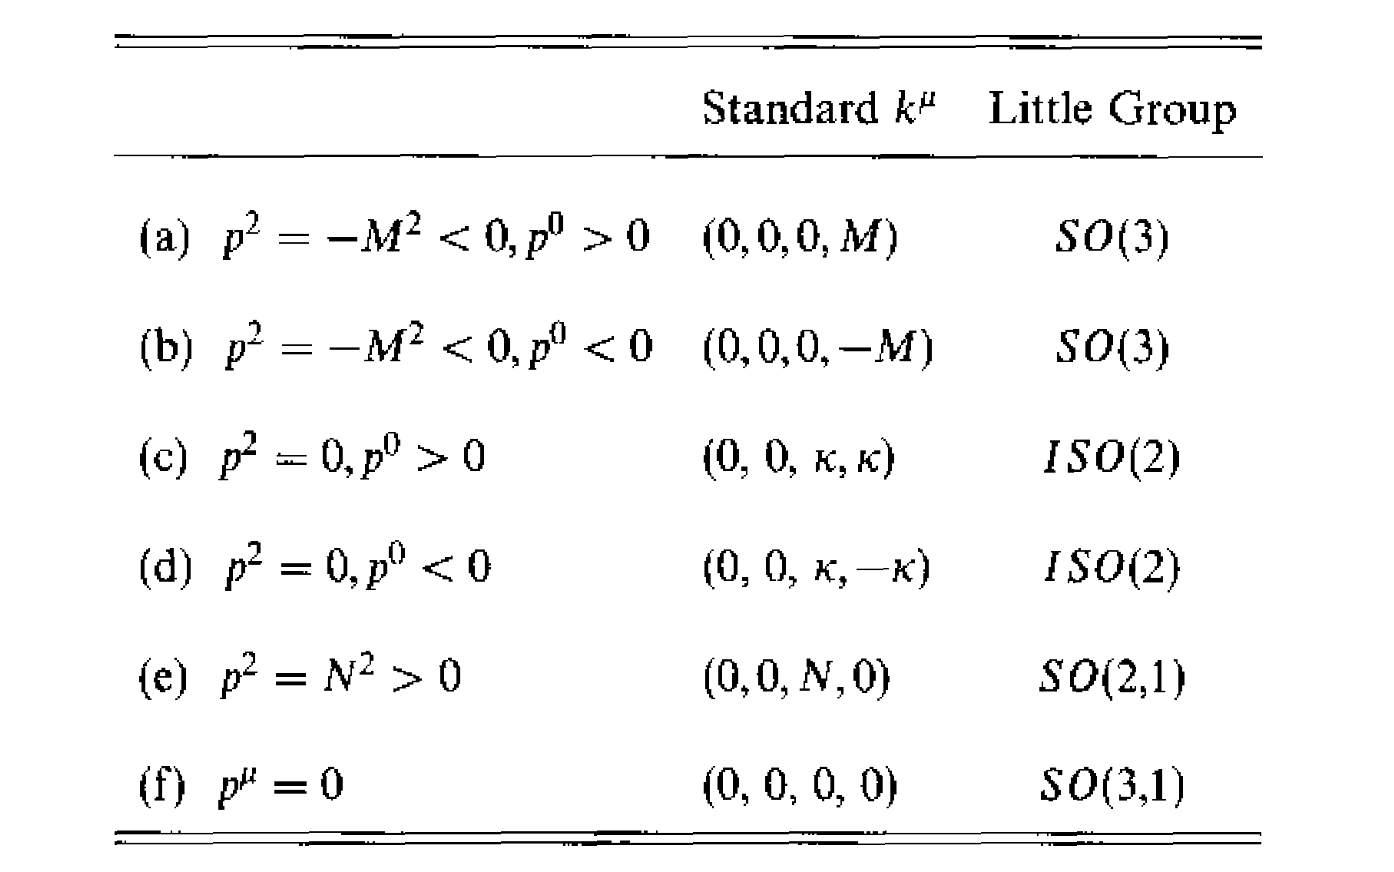
\includegraphics[width=0.85\textwidth]{2025-07-09-17-25-47.png}
        \end{center}
    \end{small}
\end{figure}
只有第一个第三个和最后一个是物理的「也就是物理上我们找到有这样的粒子」。第一个是有质量的粒子;第三个是光子;最后一个是真空。

\subsection{归一化讨论}

一般量子力学里面我们选择下面的归一化,对于\textbf{标准k矢量来说是【正交归一的】}:
\eq{
    (\Psi_{k^{\prime},\sigma^{\prime}},\Psi_{k,\sigma})=\delta^3(\mathbf{k}^{\prime}-\mathbf{k})\delta_{\sigma^{\prime}\sigma}.
}
\rmk{注意,对于\textbf{动量的本征态}来说,所有的态必须是正交的。因为动量算符是Hermite的,所以所有本征态都应该是正交态。但是\textbf{并不一定是归一的}。所以我们这里讨论的就是\textbf{归一化问题},因为正交性是Trivial的。 }
这个归一化选择的直接结果是我们的D矩阵是Unitary的矩阵:
\eq{
    D^\dagger(W)=D^{-1}(W).
}
并且考虑两个不同的单粒子态\textbf{这里是一般的p矢量}进行内积,我们有:
\eq{
    \begin{aligned}(\Psi_{p^{\prime},\sigma^{\prime}},\Psi_{p,\sigma})&=N(p)\left(U^{-1}\left(L(p)\right)\Psi_{p^{\prime},\sigma^{\prime}},\Psi_{k,\sigma}\right)\\&=N(p)N^*(p^{\prime})D\left(W(L^{-1}(p),p^{\prime})\right)_{\sigma\sigma^{\prime}}^*\delta^3(\mathbf{k}^{\prime}-\mathbf{k})\end{aligned}
}
第二步骤我们用式子\cref{eq:translaw}进行代数,其中求和因为delta符号所以没了「这里使用了不同动量本征态的正交性」。注意!我们这里 $ k' = L^{-1}(p)p' $ 是一个特别奇怪的矢量。所以我们的归一化系数$ N(p') $其实也是相对于$ k' $来说的。

我们注意到,当$ k' = k $的时候自然有$ p' = p $。而当$ p' = p $的时候,我们会发现讨论$ D\left(W(L^{-1}(p),p)\right)_{\sigma\sigma^{\prime}} $ 相当于讨论$ L(p) $变换对于$ \sigma $的影响,但是问题是所有L变换从定义上不影响$ \sigma $。所以我们的D矩阵必须是trivial的。   所以一般两个单粒子态的内积就是:
\eq{\label{eq:innerpro}
    (\Psi_{p^{\prime}\sigma^{\prime}},\Psi_{p,\sigma})=|N(p)|^{2}\delta_{\sigma^{\prime}\sigma}\delta^{3}(\mathbf{k}^{\prime}-\mathbf{k}).
}
下面我们要考虑 $ \delta^{3}(\mathbf{k}^{\prime}-\mathbf{k}) $以及$ \delta^{3}(\mathbf{p}^{\prime}-\mathbf{p}) $  的关系。为此delta函数其实是通过积分定义的,我们先需要说怎么在动量空间上面进行积分。
\imp{物理的动量空间积分}{
    物理上,我们对于动量空间进行积分的时候不能够积分完整的动量空间。因为动量空间有一些部分是非物理的,如果进行积分的话是没有任何意义的。所以我们仅仅对【可能是粒子的动量进行积分】这需要满足三个条件:
    \itm{
        \pt{粒子是on shell的也就是$ -p^2 = M^2 \geq 0 $ }
        \pt{我们只对【同一种粒子考虑积分】也就是我们积分的时候【固定粒子的质量M】}
        \pt{粒子的能量大于0也就是$ p^0 \geq 0 $ }
    }
    所以我们限制自己在这个区间内部进行积分:
    \eq{
        \begin{aligned}&\int d^4p\delta(p^2+M^2)\theta(p^0)f(p)\\=&\int d^3\mathbf{p}dp^0\delta((p^0)^2-\mathbf{p}^2-M^2)\theta(p^0)f(\mathbf{p},p^0)\\=&\int d^3\mathbf{p}\frac{f(\mathbf{p},\sqrt{\mathbf{p}^2+M^2})}{2\sqrt{\mathbf{p}^2+M^2}}\end{aligned}
    }
    这个积分第二部我们使用了delta函数的性质:
\eq{
    \delta(g(x)) = \sum_i \frac{1}{|g'(x_i)|} \, \delta(x - x_i)
\quad \text{where } g(x_i) = 0
}
我们会发现,这个要求不仅仅是我们需要限制我们的积分函数是on shell的。我们还需要有一个on shell的体积元:
\eq{
    d^3\mathbf{p}/2\sqrt{\mathbf{p}^2+M^2}.
}
这就是为什么我们量子场论使用的积分测度是:
\eq{
    \int \frac{d^3 p }{ E_p}
}
这个样子的,因为要在on shell的情况下进行积分。并且这个积分测度我们认为是\textbf{【洛伦兹不变积分测度】}因为:
\itm{
    \pt{首先,$ d^4 p  $这个积分测度应该是洛伦兹不变的。因为进行洛伦兹变换的时候变换矩阵是 $ \Lambda^\mu{}_\nu $ 这是一个行列式为1的矩阵所有Jacobi行列式是1。因此是洛伦兹不变的 }
    \pt{下面我们考虑 $ \delta(p^2+M^2)\theta(p^0) $这两个函数是洛伦兹不变的。这是显然的。 }
    \pt{根据这几个洛伦兹不变函数变换出来的积分体积元应该也是洛伦兹不变的。}
}
}

\tip{上面的测度告诉我们什么}{
    我们在相对论里,on shell的四维的积分其实可以等价于一个三维的约束下的积分。对于一个四维的标量函数的积分其实可以等价于一个三维标量函数的积分。
}
这意味着所有on shell的积分呐我们需要有这样的一个weight才能合理的进行积分。\textbf{对于全空间的积分我们可以定义delta函数是}:
\eq{
    F(\mathbf{p})=\int F(\mathbf{p}^{\prime})\delta^3(\mathbf{p}-\mathbf{p}^{\prime})d^3\mathbf{p}^{\prime}
}
下面我们想定义一个delta函数,让其在洛伦兹变换下形式不变【协变】。

由于delta函数积分结果不论任何洛伦兹变换都是1。所以delta函数积分结果永远是一个洛伦兹不变量。但问题是,积分测度$ d^3p $ 在洛伦兹变换下会进行改变的。所以我们需要一个洛伦兹不变的积分测度,因此我们形式化这么写:
\eq{
    \begin{aligned}F(p)&=\int F(\mathbf{p}^{\prime})\delta^3(\mathbf{p}-\mathbf{p}^{\prime})d^3\mathbf{p}^{\prime}\\&=\int F(\mathbf{p}^{\prime})\left[\sqrt{\mathbf{p}^{\prime2}+M^2}\delta^3(\mathbf{p}^{\prime}-\mathbf{p})\right]\frac{d^3\mathbf{p}^{\prime}}{\sqrt{\mathbf{p}^{\prime2}+M^2}}\end{aligned}
}
最后构造出来的洛伦兹不变delta函数是:
\eq{
    \sqrt{\mathfrak{p}^{\prime2}+M^2}\delta^3(\mathfrak{p}^{\prime}-\mathfrak{p})=p^0\delta^3(\mathfrak{p}^{\prime}-\mathfrak{p}).
}
因此,根据这个函数的洛伦兹不变性我们了解到:
\eq{\label{eq:transferrelation}
    \sqrt{\mathfrak{p}^{\prime2}+M^2}\delta^3(\mathfrak{p}^{\prime}-\mathfrak{p})=p^0\delta^3(\mathfrak{p}^{\prime}-\mathfrak{p}).
}
所以我们将其带入之前对于任意动量的态内积的结果的定义\cref{eq:innerpro}我们就会发现,归一化系数呈现下面的形式:
\eq{
    (\Psi_{p^{\prime},\sigma^{\prime}},\Psi_{p,\sigma})=\left|N(p)\right|^{2}\delta_{\sigma^{\prime}\sigma}\left(\frac{p^{0}}{k^{0}}\right)\delta^{3}(\mathbf{p}^{\prime}-\mathbf{p}).
}
如果我们希望归一化关系是洛伦兹不变的。那么我们可以设置归一化系数为:
\eq{
    N(p)=\sqrt{k^0/p^0}
}
这样子任意两个单粒子态进行内积的结果是:
\eq{
    (\Psi_{p^{\prime},\sigma^{\prime}},\Psi_{p,\sigma})=\delta_{\sigma^{\prime}\sigma}\delta^{3}(\mathbf{p}^{\prime}-\mathbf{p}).
}
\tip{归一化为何不唯一}{
    量子力学之中,我们的归一化方式是可以自行选取的。只要保证单粒子态在量子数不同的时候都是正交的「这是客观测量Hermite的性质决定的」。但是这个之外,我们其实有很大程度的操作自由度。因为Hilbert空间的内积其实并不一定是良好唯一定义的。

    我觉得这个值得思考慢慢讨论。
}


\rmk{
    注意我们的convension记号:
    \itm{
        \pt{当我们使用加粗的$ p $的时候,其实说的都是三维度的向量 }
        \pt{当我们写$ p_i $而不是用$ p^\mu $的时候我们考虑的都是前三个维度,并且前三个维度上下指标的数值一样!!!所以我们不区分上下指标!!  }
    }
}

\subsection{关于具体旋转变化}
之前我们讨论洛伦兹变换的时候$ x‘^\mu = \tensor{\Lambda}{^\mu_\nu}x^\nu +a^\mu $     当我们写下这个部分的时候我们使用的就是一个抽象的变换矩阵的记号。并没有给出一个具体的形式。我们考虑的是给定一个合理的$ \tensor{\Lambda}{^\mu_\nu} $矩阵我们都可以给出一个量子态的变换关系。 

一个抽象的矩阵变换关系是没有物理意义的。物理意义是人看到赋予的。比如,我们给定洛伦兹变换矩阵是一个旋转矩阵。那么,我可以翻译成这个变换【对应着观察者转动角度看到的样子】。也或许对应着物体往反向旋转看到的样子!!!

这些话都是人为翻译的。我们需要的是,把他们翻译成合理的洛伦兹变换的矩阵。那么我们现在就来看看:「物体转动$ \theta $角度对应的洛伦兹变换矩阵是什么样子的! 」

\tip{旋转矩阵具体形式}{
    学习一下呃呃呃,我真的不知道 $ \Theta_{ij} $ 是个什么东西???

    对于一般旋转来说,数学上我们的旋转矩阵的convention是这样的【注意:Weinberg用的不是这个convention】。对于绕x轴的旋转我们有:
    \[
R_x(\theta) = 
\begin{bmatrix}
1 & 0 & 0 \\
0 & \cos\theta & -\sin\theta \\
0 & \sin\theta & \cos\theta
\end{bmatrix}
\]
对于绕y轴的旋转有:
\[
R_y(\theta) = 
\begin{bmatrix}
\cos\theta & 0 & \sin\theta \\
0 & 1 & 0 \\
-\sin\theta & 0 & \cos\theta
\end{bmatrix}
\]
【注意我们右手系的顺序是,123,所以看看$ -sin\theta $在哪个位置!! 】对于绕z轴的旋转有:
\[
R_z(\theta) = 
\begin{bmatrix}
\cos\theta & -\sin\theta & 0 \\
\sin\theta & \cos\theta & 0 \\
0 & 0 & 1
\end{bmatrix}
\]
\line
对于一般旋转就是这样的三个旋转的组合所以就是:
    \textbf{Rodrigues 公式(绕单位轴 $\hat{n} = (n_1, n_2, n_3)$ 旋转角度 $\theta$):}
\[
R(\hat{n}, \theta) = I + \sin\theta\, K + (1 - \cos\theta)\, K^2
\]
其中 $K$ 是 $\hat{n}$ 的反对称张量形式:
\[
K = 
\begin{bmatrix}
0 & -n_3 & n_2 \\
n_3 & 0 & -n_1 \\
-n_2 & n_1 & 0
\end{bmatrix}
\]
\line

对于无穷小的转动,我们有将$ \theta \to 0 $在这样的极限下面我们有: 
\[
R(\boldsymbol{\theta}) \approx I + \theta^i J_i + \mathcal{O}(\theta^2)
\]
这就是无穷小旋转矩阵。其中:
\[
J_1 =
\begin{bmatrix}
0 & 0 & 0 \\
0 & 0 & -1 \\
0 & 1 & 0
\end{bmatrix}, \quad
J_2 =
\begin{bmatrix}
0 & 0 & 1 \\
0 & 0 & 0 \\
-1 & 0 & 0
\end{bmatrix}, \quad
J_3 =
\begin{bmatrix}
0 & -1 & 0 \\
1 & 0 & 0 \\
0 & 0 & 0
\end{bmatrix}
\]
% 这样子给出的$ \Theta_{ij} $【Weinberg之中定义的】正好$ \Theta_{ij} = -\epsilon_{ijk}\theta_k $这个产生了一个负号就很不好。

}
% \imp{Weinberg的convention讨论}{
%     所以Weinberg使用了另一个convention,也就是写出的标准旋转矩阵不一样。就是把所有这些矩阵都取了转置,这样子我们的convention的结果是:$ \Theta_{ij} = +\epsilon_{ijk}\theta_k  $「所以下面这个大写的$ \Theta $其实就是列举出来了绕着每一个轴转动的角度!!!」 
% \bigskip

%     Weinberg之中定义这样的矩阵才是标准的旋转矩阵。所以下卖弄我们提及标准的旋转矩阵都是上面的矩阵的转置:
%     \eq{
%         R(\theta)\equiv\begin{bmatrix}\cos\theta&\sin\theta&0&0\\-\sin\theta&\cos\theta&0&0\\0&0&1&0\\0&0&0&1\end{bmatrix}
%     }
% }
% \line
% 下面我们复习一下群表示论SO(3)群的有限维不可约表示是怎么通过SO(3)群的群元素构造出来的。


Weinberg的convention和这个相差了一个转置。但这没有什么意义,就是写一个矩阵而已。这么写矩阵有个好处,就是作一阶展开的时候,下面定义的$ \Theta_{ij} $都是正的,也就是$ \Theta_{ij} = \theta_k \epsilon_{ijk} $  其中$ \theta $是以顺时针为正方向「也就是转置之后」 的变化角度$ \theta $。 


\subsection{正质量粒子}
对于正质量的粒子来说little group是SO(3)群,也就是我们的三维的旋转群\hlr{「这很合理,因为三个维度怎么转必然不影响第四个维度的M,也就是没有Boost的纯转动群」}。所以当我们考虑单粒子态的Hilbert空间的矢量在Lorentz变换下面的运动的时候,如果我们具体写出来:
\eq{\label{eq:translaw}
    U(\Lambda)\Psi_{p,\sigma}=\left(\frac{N(p)}{N(\Lambda p)}\right)\sum_{\sigma^{\prime}}D_{\sigma^{\prime}\sigma}\left(W(\Lambda,p)\right)\Psi_{\Lambda p,\sigma^{\prime}}.
}
其中归一化我们选择 $ N(p)=\sqrt{k^0/p^0} $。我们知道:$ D_{\sigma^{\prime}\sigma}\left(W(\Lambda,p)\right) $ 是SO(3)群的有限维不等价不可约表示。

\line
为了计算 $ D_{\sigma^{\prime}\sigma}^{(j)}\left(W(\Lambda,p)\right) $ 
\hlr{我们需要解决两个问题:}
\itm{
    \pt{这个样子的洛伦兹变换到底对应了什么量子矩阵$ U(W)$ }
    \pt{哪一个W的元素对应了$ L^{-1}(\Lambda p)\Lambda L(p) $也就是,$ W(\Lambda,p) $洛伦兹变换呈现什么样子? }
}
\imp{回答第一个问题,SO(3)群表示}{
    数学上的研究告诉我们,SO(3)群的表示可以用 $ j = 0,1/2,1,3/2... $进行label,并且表示是$ d = 2j+1 $的。对于一个\textbf{无限小的转动} $ R $,显然这个是W群的元素也是洛伦兹群的一个元素,我们的D矩阵可以写出具体的数值。旋转矩阵:$ R_{ij} = \delta_{ij}+\Theta_{ij} $ 其中$ \Theta_{ij}  = -\Theta_{ji}$ 。这个矩阵应该是一个合理的洛伦兹变换的矩阵之中空间旋转的某一个。

表示满足下面的关系:
\eq{\label{eq:Dtrans}
    \begin{aligned}D_{\sigma^{\prime}\sigma}^{(j)}(1+\Theta)&=\delta_{\sigma^{\prime}\sigma}+\frac{i}{2}\Theta_{ik}(J_{ik}^{(j)})_{\sigma^{\prime}\sigma},\end{aligned}
}
这里面,我们使用了一个J算符定义是:
\eq{
    (J_{23}^{(j)}\pm iJ_{31}^{(j)})_{\sigma^{\prime}\sigma}&=(J_1^{(j)}\pm iJ_2^{(j)})_{\sigma^{\prime}\sigma}\\&=\delta_{\sigma^{\prime},\sigma\pm1}\sqrt{(j\mp\sigma)(j\pm\sigma+1)},\\(J_{12}^{(j)})_{\sigma^{\prime}\sigma}&=(J_3^{(j)})_{\sigma^{\prime}\sigma}=\sigma\delta_{\sigma^{\prime}\sigma},
}
其中$ \sigma $的取值是$ -j, -j+1,..., j-1,j $ 。

\rmk{上面给出的是无限小的变换,但是,我们知道,绕某一个方向转动都是Abelian的,所以都可以写成$ U(R_i(\Theta_{jk})) = e^{(i/2 )\Theta_{jk} J^m_{jk}} $ 的形式。然后根据D矩阵的复合关系\cref{eq:littlegroupcom}我们可以知道,任何转动其实都是绕x轴转动和z轴转动的复合。所以就可以求出来一般的转动的结果了。}
}


\imp{回答第二个问题}{

    \textbf{\hlr{STEP 1:}} 
    首先,我们必须fix一个standard momentum。对于有质量的粒子,我们一般选择$ k^\mu = (0,0,0,M) $这个向量。
    \bigskip

    \textbf{\hlr{STEP 2:}}
    下面我们给出一个\textbf{标准的$ L(p) $ Boost形式 }。显然$ L(p) $并不是唯一选取的,我们需要进行一个合理规定:
    \eq{
        \begin{aligned}
  & L^{i}{}_{k}(p) = \delta_{ik} + (\gamma - 1) \hat{p}_{i} \hat{p}_{k}, \\
  & L^{i}{}_{0}(p) = L^{0}{}_{i}(p) = \hat{p}_{i} \sqrt{\gamma^{2} - 1}, \\
  & L^{0}{}_{0}(p) = \gamma,
\end{aligned}
    } 
    其中参数是:
    \eq{
        \hat{p}_i\equiv p_i/|\mathbf{p}|,\quad\gamma\equiv\sqrt{\mathbf{p}^2+M^2}/M
    }
有了这些规则,我们可以从定义计算出每一个$ \Lambda $以及p对应的Little Group了! 
\bigskip

\textbf{\hlr{STEP 2(exception):}}
我们进行一个观察,发现,对于三维度的空间旋转变换也就是$ \tensor{\Lambda}{^\mu_\nu} $是仅仅有三维空间旋转变换,我们记作$ \mathscr{R} $ 。Little group的元素本身就是对应的$ W = \mathscr{R} $。就是这两个矩阵是一模一样的:
\eq{
    W(\mathscr{R},p)=\mathscr{R}
}
【证明请回去看Weinberg pg 69】
\bigskip 

}
\rmk{所有W的元素其实都是三维度转动的元素之一,不论$ W(\Lambda,p) $里面的$ \Lambda $是什么洛伦兹变换。但是,如果刚好$ \Lambda $没有boost就是一个三位的旋转变换,那么无论$ p $的取值是多少都满足:$  W(\mathscr{R},p)=\mathscr{R} $ 。   

因此,相对论的有质量的粒子的旋转变换下的变换关系和naively我们规定的量子力学的SO(3)群表示的变换关系是一模一样的。我们可以直接从非相对论的量子力学的东西挪过去。

}

所以我们知道对于一个质量$ M > 0 $并且 spin j的粒子来说,洛伦兹变换作用在量子态上面呈现为:
\eq{
    U(\Lambda)\Psi_{p,\sigma}=\sqrt{\frac{(\Lambda p)^0}{p^0}}\sum_{\sigma^{\prime}}D_{\sigma^{\prime}\sigma}^{(j)}\left(W(\Lambda,p)\right)\Psi_{\Lambda p,\sigma^{\prime}},
}   
【我们这里使用之前的那个归一化!!】并且注意little group的元素定义是:
\eq{
    W(\Lambda,p)=L^{-1}(\Lambda p)\Lambda L(p).
}






\subsection{无质量粒子}

同样的我们需要研究这个Little Group是个什么。我们一般选择的标准4动量是:$ k^\mu = (0,0,1,1) $,所以根据Little Group的定义就是那些满足$ \tensor{W}{^\mu_\nu}k^\nu = k^\mu $的洛伦兹变换矩阵。我们考虑这样的矩阵需要满足什么性质。数学上我们意识到这样的矩阵作用在另外的一个向量$ t^\mu = (0,0,0,1) $上面需要满足下面的性质:
\eq{
    (Wt)^\mu(Wt)_\mu=t^\mu t_\mu=-1,\\(Wt)^\mu k_\mu=t^\mu k_\mu=-1.
}
满足第二个条件的矩阵我们知道可以写作下面形式:
\eq{
    (Wt)^\mu=(\alpha,\beta,\zeta,1+\zeta)
}
然后我们把这个ansatz带入第一个式子,我们得到:
$ \zeta = (\alpha^2+\beta^2)/2 $
所以我们会发现,满足下面两个条件\hlr{1. 是一个lorentz transformation矩阵};\hlr{2.作用在(0,0,0,1)和(0,0,1,1)向量上面结果是对的}。这完全决定了一个矩阵的形式是:
\eq{\label{eq:Smatrixlorentz}
    S^{\mu}{}_{\nu}(\alpha,\beta)=\begin{bmatrix}1&0&-\alpha&\alpha\\0&1&-\beta&\beta\\\alpha&\beta&1-\zeta&\zeta\\\alpha&\beta&-\zeta&1+\zeta\end{bmatrix}.
}
但这不意味着S就是W。这仅仅告诉我们,将$ S^{-1} W $作用在$ k^\mu $以及$ t^\mu $向量上面会使其不变。所以,我们会发现W其实有更多的自由度,就是绕着第三个维度进行旋转的自由度,由于洛伦兹变换的要求,所以只能是旋转矩阵:
\eq{
    S^{-1}(\alpha,\beta)W=R(\theta),
}
其中旋转矩阵的样子大概是:
\eq{\label{eq:Rmatrixrotate}
    \left.R^\mu{}_v(\theta)\equiv\left[\begin{array}{cccc}\cos\theta&\sin\theta&0&0\\-\sin\theta&\cos\theta&0&0\\0&0&1&0\\0&0&0&1\end{array}\right.\right].
}
\imp{无质量粒子的Wigner Little Group元素}{
    因此,我们可以定义无质量粒子的Wigner Little Group的形式就是:
    \eq{
        W(\theta,x,\beta)=S(x,\beta)R(\theta)\mathrm{~.}
    }
    其中涉及的两个洛伦兹变换矩阵是:\cref{eq:Smatrixlorentz,eq:Rmatrixrotate}。我们分析这个群的结构。我们意识到:
    \itm{
        \pt{S和R矩阵,独立的构成的都是Abelian的群。 也就是说独立的复合关系是:}
        \eq{\label{eq:composerule}
            S(\bar{\alpha},\bar{\beta})S(\alpha,\beta)&=S(\bar{\alpha}+\alpha,\bar{\beta}+\beta),\\
R(\bar{\theta})R(\theta)&=R(\bar{\theta}+\theta).    
        }
        \pt{仅仅有S构成的群是一个\hlr{不变子群},也就是整个大的群任意元素变换S子群的元素结果都是S子群的元素。具体的写出来就是:}
\eq{\label{eq:invarianttrans}
    R(\theta)S(\alpha,\beta)R^{-1}(\theta)=S(\alpha\cos\theta+\beta\sin\theta,-\alpha\sin\theta+\beta\cos\theta).
}
    }
    根据这个性质,我们可以计算出所有群元素的乘积的复合关系。这个群正是ISO(2)群。
}
从群论的视角,\hlr{所有没有Invariant(不变的) Abelian Subgroup的群都是半单的}。所以我们知道,ISO(2)群显然比较复杂。我们考虑这个群的李代数。由于这个群是洛伦兹群的子群,所以我们显然可以进行一个无限小的展开:
\begin{equation}
\begin{aligned}
    &W(\theta,\alpha,\beta)^{\mu}{}_{\nu} = \delta^{\mu}{}_{\nu} + \omega^{\mu}{}_{\nu}, \\
    &\omega_{\mu\nu} = 
    \begin{bmatrix}
        0 & \theta & -\alpha & \alpha \\
        -\theta & 0 & -\beta & \beta \\
        \alpha & \beta & 0 & 0 \\
        -\alpha & -\beta & 0 & 0
    \end{bmatrix}.
\end{aligned}
\end{equation}
我们之前定义的洛伦兹变换如果写成上面式子这样的形式,那么量子的洛伦兹变换的展开应该呈现:\cref{eq:expansions}。所以我们自然知道这个群的量子的洛伦兹变换呈现:
\eq{
    U(W(\theta,x,\beta))=1+i\alpha A+i\beta B+i\theta J_3
}
其中:
\eq{
    A=-J^{13}+J^{10}=J_2+K_1,\\
    B=-J^{23}+J^{20}=-J_1+K_2,
}
其中,我们知道三维的两个反对称指标可以使用一个指标进行表示。我们的convention是$ J_{ij} = \epsilon_{ijk}J_k $。根据我们之前推出的洛伦兹变换生成元的对易关系:\cref{eq:commutationrelation}我们知道: 
\eq{
    \begin{aligned}&[J_3,A]=+iB,\\&[J_3,B]=-iA,\\&[A,B]=0.\end{aligned}
}
我们会发现原来A,B是两个互相对易的算符,所以我们可以用这两个算符的一组共同本征值作为量子态的label,$ \Psi_{k,a,b} $:
\eq{
    A\Psi_{k,a,b}=a\Psi_{k,a,b},\\
B\Psi_{k,a,b}=b\Psi_{k,a,b}.
}
但是同时根据\cref{eq:invarianttrans}我们知道,如果对于算符A,B作用上量子的转动变换我们可以得到:
\eq{
    \begin{aligned}U[R(\theta)]AU^{-1}[R(\theta)]&=A\cos\theta-B\sin\theta,\\U[R(\theta)]BU^{-1}[R(\theta)]&=A\sin\theta+B\cos\theta,\end{aligned}
}
所以说,对于任意的一个非0的A,B本征态的量子态。我们其实是可以通过转动生成无限多个本征态的,我们标记为$ \Psi^\theta_{k,a,b} $。\hlr{注意:这个量子态并不是转动的J的本征态仅仅是拿一个转动角度标记的量子态。} 这一系列量子态的本征值是:
\eq{
    A\Psi_{k,a,b}^\theta=(a\cos\theta-b\sin\theta)\Psi_{k,a,b}^\theta,\\
    B\Psi_{k,a,b}^\theta=(a\sin\theta+b\cos\theta)\Psi_{k,a,b}^\theta,
}
并且和原本的量子态的关系是:
\eq{
    \Psi_{k,a,b}^{0}\equiv U^{-1}\left(R(\theta)\right)\Psi_{k,a,b}.
}
\hlr{但问题是我们在实验上面并没有发现没有质量的粒子存在这样连续的量子态。}所以我们下面给出真正的物理的Hilbert空间:
\imp{无质量粒子的Hilbert空间}{
    无质量的粒子所在Hilbert空间是A,B算符本征值为0的Hilbert子空间。由于对于这个空间来说,A,B从算符退化为了一个具体的数字0。所以对于这个空间来说$ J_3 $其实和A,B算符是对易的,可以有共同本征值,我们记为$ \Psi_{k,\sigma} $  
    
    这个空间之中的向量满足:
    \eq{
        A\Psi_{k,\sigma}=B\Psi_{k,\sigma}=0\mathrm{~.}\\
        J_3\Psi_{k,\sigma}=\sigma\Psi_{k,\sigma}.
    }
    \hlr{注意,我们之前定义的标准的k是(0,0,1,1),所以,sigma是绕着k方向的转动}。也就是绕着运动方向转动的角动量,被称为Helicity!
}
\line
我们上面确认了无质量粒子的Hilbert空间是什么。下面,我们计算一般的Lorentz变换下面无质量粒子是怎么变换的。对于Little Group之外的变换就是\cref{eq:separa}里面这样使用L直接对于动量进行变换。还是那两个问题:
为了计算 $ D_{\sigma^{\prime}\sigma}^{(j)}\left(W(\Lambda,p)\right) $ 
\hlr{我们需要解决两个问题:}
\itm{
    \pt{这个样子的洛伦兹变换到底对应了什么量子矩阵$ U(W)$ }
    \pt{哪一个W的元素对应了$ L^{-1}(\Lambda p)\Lambda L(p) $也就是,$ W(\Lambda,p) $洛伦兹变换呈现什么样子? }
}

\imp{回答第一个问题,两个子群的表示}{
    首先,作为Abelian的子群我们可以写作:
\eq{
    U(S(\alpha,\beta))=\exp(i\alpha A+i\beta B)\\
    U(R(\theta))=\exp(iJ_3\theta)\mathrm{~.}
}
所以对于一个洛伦兹变换可以写成这两个变换的复合,然而根据\cref{eq:littlegroupcom}我们的little group的元素的乘法体现在U表示上也是直接乘法。
\eq{
    U(W)\Psi_{k,\sigma}=\exp(i\alpha A+i\beta B)\exp(i\theta J_3)\Psi_{k,\sigma}=\exp(i\theta\sigma)\Psi_{k,\sigma}
}
因此我们的D矩阵形式化的可以表达为:
\eq{
    D_{\sigma^{\prime}\sigma}(W)=\exp(i\theta\sigma)\delta_{\sigma^{\prime}\sigma},
}
整体写出变换规则就是:
\eq{
    U(\Lambda)\Psi_{p,\sigma}=\sqrt{\frac{(\Lambda p)^0}{p^0}}\exp\left(i\sigma\theta(\Lambda,p)\right)\Psi_{\Lambda p,\sigma}
}
这下我们回答了第一个问题。
}

\imp{回答第二个问题}{
    而对于第一个问题,我们讨论$ \theta(\Lambda,p) $到底怎么求解。就是反向解这个方程:
\eq{
    W(\Lambda,p)\equiv L^{-1}(\Lambda p)\Lambda L(p)\equiv S\left(\alpha(\Lambda,p),\beta(\Lambda,p)\right)R\left(\theta(\Lambda,p)\right).
}
注意,我们这里是规定convention的。所有的S,R矩阵需要是和上面对应:\cref{eq:Smatrixlorentz,eq:Rmatrixrotate}。

\rmk{我们之后意识到$ \alpha,\beta $和规范对称性有关系。然后,这里看起来$ \sigma $的取值应该是连续实数的,后面我们会意识到这个只能去正整数或者半正整数。}

为了能够反解决这个方程我们依旧需要一个标准的$ L(p) $洛伦兹变换,把$ k^\mu = (0,0,\kappa,\kappa) $变换成任意的四矢量$ p^\mu $。就像有质量的粒子一样,但是这里我们使用的是:
\eq{
    L(p)=R(\mathbf{\hat{p}})B(|\mathbf{p}|/\kappa)
} 
其中矩阵B是:
\eq{
    \left.B(u)\equiv\left[\begin{array}{cccc}1&0&0&0\\0&1&0&0\\0&0&(u^2+1)/2u&(u^2-1)/2u\\0&0&(u^2-1)/2u&(u^2+1)/2u\end{array}\right.\right]
}
\rmk{再次提醒我们的convension,对于$ \mathbf{p} $我们的意思是只考虑空间的三维的情况!!!$ p_i $也是!!  }
其中矩阵R是一个纯粹的转动矩阵,把第三个坐标轴(0,0,1)转动到p的运动的方向。我们假设粒子p的方向是$ \mathbf{\hat{p}}=\left(\sin\theta\cos\phi,\sin\theta\sin\phi,\cos\theta\right). $ 然后,我们可以知道,把一个$ (0,0,1) $向量变成这个样子分为两个步骤:
\itm{
    \pt{绕着第二个轴转$ \theta $角度 }
    \pt{绕着第三个轴再转$ \phi $ 角度}
} 
所以这一波操作对应的洛伦兹变换【注意是洛伦兹变换,毕竟R也是个洛伦兹变换矩阵。并不是Little Group的表示】是:
\eq{
    U(R(\hat{\mathbf{p}}))=\exp(i\phi J_3)\exp(i\theta J_2)\mathrm{~,}
}

}
讨论一下关于helicity,显然不同helicity的粒子应该是不同的粒子。因为helicity并不会因为洛伦兹变换而改变。但是,我们之后会发现,相反helicity的粒子是可以通过空间反向对称性相关联的。但是beta辐射之中产生的neutrinos和antineutrinos似乎是两种不同的粒子。

由于相反Helicity的粒子被认为是同样的粒子。所以我们可以进行一波叠加,才能形成一个一般的单粒子态。比如对于一个单光子态来说:
\eq{
    \Psi_{p,\alpha}=\alpha_+\Psi_{p,+1}+2\alpha_-\Psi_{p,-1},
}
其中系数需要满足$ |x_{+}|^{2}+|x_{-}|^{2}=1. $所以我们的光存在圆偏振和椭圆偏振的现象。 

\tip{总结怎么计算量子洛伦兹变换}{
    整个计算分为两步:
    \itm{
        \pt{\hlr{第一步} 计算洛伦兹变换对应的Little Group【写成矩阵,洛伦兹群的子群】的元素是什么}
        \pt{\hlr{第二步} 根据Little Group的元素,带入量子洛伦兹变换的公式计算D矩阵。}
        \pt{最后整体写开就好了!!}
    }
}




\section{时间和空间反演变换}
我们上面讨论的都是一个小小的1附近的(proper and orthochronous)洛伦兹群。下面我们考虑两个大大的变换带来的影响。一切其他的洛伦兹群都可以通过$ \mathscr{P} $以及$ \mathscr{T} $ 或者组合的$\mathscr{PT} $变换得到。这两个变换的矩阵是:
\eq{
    \left.\mathscr{P}_\nu^\mu=\left[\begin{array}{rrrr}-1&0&0&0\\0&-1&0&0\\0&0&-1&0\\0&0&0&1\end{array}\right.\right],\quad\mathscr{F}_\nu^\mu=\begin{bmatrix}1&0&0&0\\0&1&0&0\\0&0&1&0\\0&0&0&-1\end{bmatrix}.
}  
根据洛伦兹变换的复合关系\cref{eq:quantumlorentz},我们可以知道,包含TP作用的洛伦兹群也应该满足这个关系。我们假设TP也有自己对应的作用在Hilbert空间上面的算符:
\eq{
    \mathsf{P}\equiv U\left(\mathscr{P},0\right)\quad\mathsf{T}\equiv U\left(\mathscr{T},0\right)
}
似的这个算符的作用满足类似于\cref{eq:quantumlorentz}的关系,我们定义TP算符作用在洛伦兹群对应的算符上面的结果是:
\eq{
    \begin{aligned}\mathsf{P}U\left(\Lambda,a\right)\mathsf{P}^{-1}&=U\left(\mathscr{P}\Lambda\mathscr{P}^{-1},\mathscr{P}a\right),\\\mathsf{T}U\left(\Lambda,a\right)\mathsf{T}^{-1}&=U\left(\mathscr{T}\Lambda\mathscr{T}^{-1},\mathscr{T}a\right)\end{aligned}
}
\hlr{注意,上面的式子是“定义式”,但是是“合理的”。考虑到Lorentz群本身的复合关系。}



% 这里我们记录我们为了读懂文章需要补充的知识点。

% \idea{一个你太难伟大的想法}{
%     这就是我的想法捏!
% }

% \ques{问题呀}{
%     这是一个问题呀!
%     \itm{
%         \pt{\textbf{这个问题一个解决思路就是}}
%     }
% }
% \imp{一个重要的内容}{
%     这是一个重要的内容!
% }

% \conclusion{%
% 这是一个重要的结论。我们证明了该定理成立,并且可以应用于多个场景。
% }

% \attention{%
% 请特别注意,这里的假设条件是关键,否则后续结论不成立。
% }

% \tip{%
% 使用这个技巧可以大大简化计算过程,提升效率。
% }

% \questionbox{%
% 该问题的关键难点在于理解边界条件的选择,欢迎大家讨论。
% }